\subsection{Geographic Engine}\label{comp:geographicEngine}
\begin{figure}[H]
	\centering
	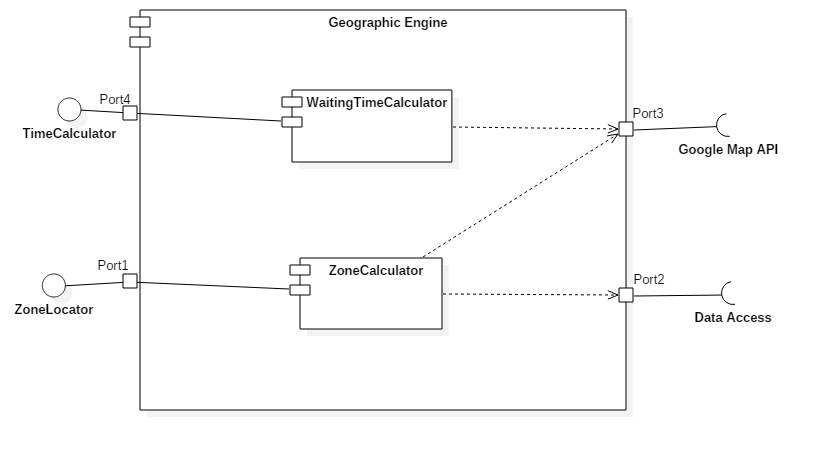
\includegraphics[scale=0.5]{../"Analysis Documents"/components/geographicEngine}
	\label{fig:geographicengine}
	\caption{Geographic Engine internal structure}
\end{figure}
\subsubsection{Provided interfaces}
\begin{table}[H]
	\begin{longtable}{| p{0.3\textwidth} | p{0.3\textwidth} | p{0.4\textwidth} |}
		\hline
		\textbf{Provided Interface} & \textbf{Dedicated user} & \textbf{Description} \\ \hline
		TimeCalculator & Ride Manager component & Given a source location and a destination, it calculates an approximative waiting time \\ \hline
		ZoneLocator & Taxi Manager, Queue Manager and Ride Manager components & It calculates the corresponding zone of a given location if it is valid (being valid means to be inside the city) \\ \hline
	\end{longtable}
	\caption{Geographic Engine: provided interfaces}
	\label{tab:geographicengine:providedInterfaces}
\end{table}
\subsubsection{Required interfaces}
\begin{table}[H]
	\begin{longtable}{| l | p{.80\textwidth} |}
		\hline
		\textbf{Required Interface} & \textbf{Description and usage} \\ \hline
		Google Maps API & Used for the activity of geocoding and for calculating the approximative travel time \\ \hline
		DataAccess & Retrieve the information about taxi zones \\ \hline
	\end{longtable}
	\caption{Geographic Engine: required interfaces}
	\label{tab:geographicengine:requiredInterfaces}
\end{table}
